%% HMRS platform — Knowledge-Based Systems submission (elsarticle)
%% v3 restructure 2026-11-11: hierarchical *management* framing — the system
%% manages documents at three levels (collection / document / segment) and
%% serves a tiered access path; retrieval algorithms are supporting components.
%% 20-page pass 2026-10-13: back matter (n_back) included; figures restored.
%% Compile: pdflatex main_20p && bibtex main_20p && pdflatex main_20p && pdflatex main_20p
%% AUTHOR ACTION (authors reserved these values; do not infer them):
%%   1. frontmatter below: author names/order, affiliation, city, country,
%%      corresponding-author e-mail, and the ORCID lines if any;
%%   2. n_back.tex: the two CRediT names, the funding wording and the
%%      acknowledgements;
%%   3. n_back.tex: confirm the generative-AI declaration (service names are
%%      filled; versions only if the editors ask).
%% This is a double-column review preview with a local 20-page target.
%% The exact KBS submission layout remains subject to its author guide.
% journal-style camera-ready preview (generated from the submission sources)
\documentclass[final,5p,times,twocolumn]{elsarticle}
\usepackage{stfloats}

\usepackage[T1]{fontenc}
\usepackage[utf8]{inputenc}
\usepackage{booktabs}
\usepackage{array}
\usepackage{graphicx}
\usepackage{amsmath}
\usepackage{amssymb}
\usepackage{xcolor}
\usepackage{url}
\usepackage[colorlinks=true,linkcolor=blue,citecolor=blue,urlcolor=blue]{hyperref}
\usepackage{xurl}
\urlstyle{same}
% DOIs are emitted by the .bst as \path{...}; re-declare it so they
% typeset in the ambient roman face at 7.2 pt instead of 6.97 pt typewriter.
\DeclareUrlCommand\path{\urlstyle{same}}
\usepackage{caption}
\captionsetup{font=small,labelfont=bf}
\usepackage{algorithm}
\usepackage{algpseudocode}
\newcommand{\yes}{\checkmark}
\newcommand{\no}{--}

\graphicspath{{figs/}}
\setlength{\emergencystretch}{1.5em}

%% Float placement: the paper carries eight figures and seven body table
%% environments (Figure 10 was removed on 2026-10-17 because Table 5 carries
%% the same six methods; the five appendix tables moved to the supplementary
%% material on 2026-10-16), so the
%% default fractions defer most of them past the references. Allow denser
%% float pages to keep each float near the text that discusses it.
\renewcommand{\topfraction}{0.90}
\renewcommand{\bottomfraction}{0.85}
\renewcommand{\textfraction}{0.08}
\renewcommand{\floatpagefraction}{0.75}
\renewcommand{\dbltopfraction}{0.90}
\renewcommand{\dblfloatpagefraction}{0.75}
\setcounter{topnumber}{3}
\setcounter{bottomnumber}{2}
\setcounter{totalnumber}{4}
\setcounter{dbltopnumber}{3}

%% Tighten the vertical glue around floats. With nine figures and twelve
%% tables the elsarticle defaults spend roughly three inches of column
%% height on separation alone, which the 20-page budget cannot afford.
%% Values are about half the class defaults and remain within normal
%% typographic practice for a two-column layout.
\setlength{\floatsep}{7pt plus 2pt minus 2pt}
\setlength{\textfloatsep}{9pt plus 2pt minus 2pt}
\setlength{\intextsep}{7pt plus 2pt minus 2pt}
\setlength{\dblfloatsep}{7pt plus 2pt minus 2pt}
\setlength{\dbltextfloatsep}{9pt plus 2pt minus 2pt}

\journal{Knowledge-Based Systems}

\begin{document}

\begin{frontmatter}

\title{HMRS: A hierarchical management-and-retrieval system for tiered
knowledge document organisation and evidence-traced access}

\author[inst1]{Author Name\corref{cor1}}
\ead{author@example.com}
\author[inst1]{Co-author Name}
\cortext[cor1]{Corresponding author.}
\affiliation[inst1]{organization={Affiliation Department, University,
City, Country}, city={City}, country={Country}}

\begin{abstract}
A document collection becomes a knowledge base only when its documents are
parsed, classified into the owning collection, kept consistent as it changes,
and searched there. We present HMRS (Hierarchical Management Retrieval
System), a self-hosted knowledge document management system that manages
documents at three levels---collection, document and segment---and answers
questions along a tiered path narrowing from the catalogue of collections,
through document descriptions, to the segment carrying the evidence.
Classification derives from the parsed body rather than the filename, and the
shelf tier exposes descriptions before any body is read. At the segment tier,
evidence is admitted under an optional gate, and enforced checks are kept
separate from workflow decisions.
On a 100-paper snapshot, 79 papers were retrievable and 21 not; cross-lingual
membership was 0.875 (EN) and 1.0 (ZH/JA). A 72-question
scripted route audit returned the gold collection for 72/72 versus 37/72
with nominally name-only cards; an unlogged fallback may use descriptions. On the same questions, the tiered path with a chunk-window evidence
union contained the gold string in 52/72 (72.2\%), above a
flat union with a reference-mode judge (39/72) and above a
navigation-free precise arm (46/72). The configurations differ in multiple
components, and a gold-label-dependent lookup limits the flat comparison. The answer or recorded
trace contained a gold identifier in all 60 grid cells, and verifier-score re-ranking lowered Hit@5 from
0.94 to 0.44 while fusion order restored 0.94. These results demonstrate an
auditable management structure with independent per-tier measurements and warn
against verifier-as-ranker; they do not establish general retrieval superiority
or semantic answer quality. These findings suggest that a managed, auditable
collection is a practical, inspectable basis for evidence-traced knowledge
bases.
\end{abstract}

\begin{keyword}
Knowledge document management \sep Document classification \sep
Hierarchical organisation \sep Tiered retrieval \sep Evidence verification \sep
Model Context Protocol
\end{keyword}

\end{frontmatter}

%% ============================================================ body (v2 order)
\section{Introduction}
\label{sec:intro}

Enterprises record regulations, failure analyses and operational lessons in
unstructured documents. A document collection becomes a knowledge base only
when its documents are parsed and admitted reliably, classified into the
collections that own them and kept consistent as those collections change.
A question must then be answerable by moving down a path from the collection
to the document and finally to the passage that carries the evidence.
Answering a question such as \emph{why did edge delamination appear in a
photovoltaic inspection?} requires the collection that holds inspection
reports, the report that records the decision, the passage inside it and an
accurate pointer to both.

The two capabilities required for this operate on different parts of the
lifecycle. Modular RAG and agentic-retrieval surveys already treat indexing
and pre-retrieval as first-class pipeline modules
\cite{modular-rag,gao-ragsurvey}; what remains separated is the governance of
the collection itself---its placement, lifecycle and per-tier audit---from
the retrieval step that consumes it. Content-based
retrieval addresses the query step within a collection that is already
indexed: retrieval-augmented generation (RAG) embeds queries and passages in
a shared vector space \cite{rag-lewis,dpr}, agentic systems let a language
model call retrieval tools \cite{mcp,singh-agentic-rag}, and hybrid, lexical
and graph-structured variants extend the ranking model
\cite{bm25,rrf-cormack,graphrag,lightrag,raptor}. Knowledge management
addresses the collection itself: enterprise content management governs
organisational documents \cite{paivarinta-ecm-2005,tyrvaainen-ecm-2006},
metadata and tagging studies ask how documents are described and reviewed
\cite{park-metadata-quality-2009,golder-tagging-2006}, and public knowledge
bases curate facts under explicit ontologies
\cite{auer-dbpedia-kb-2007,hoffart-yago2-kb-2013}. Semantic similarity
measures topical relatedness rather than evidence containment, a failure mode
discussed in the hallucination and RAG surveys \cite{siren,gao-ragsurvey}.
A correctly ranked passage is
likewise unreachable when the collection that owns it was never classified, was filed
under a name that does not match its content, or was indexed after a rename
that left the index stale.

This separation creates a systems problem at the boundary between the two
streams. A collection can be perfectly indexed and the system still answer wrongly,
because the first decision a question requires---which collection to
consult---is made without reference to the collection structure in flat,
single-index deployments.
Distributed IR has long studied this collection-selection step
\cite{callan1995searching,si2003redde}, but models collections as static
statistical summaries rather than as managed state that is written to and
checked by reconciliation audits after selected lifecycle operations.
Conversely, a carefully curated hierarchy does not help when no tiered
procedure carries a question from the catalogue down to the evidence. The
question we study is therefore not how to rank passages better, but how a
document collection should be \emph{managed} so that a query can be served
tier by tier---selecting a collection, then a document, then a segment---and
so that each tier can be audited independently. We study that question through
an implemented system and bounded operational audits. Integration by itself is
not treated as evidence of improved retrieval or answer quality.

HMRS (Hierarchical Management Retrieval System) is a self-hosted
knowledge document management system. It maintains collections, documents and
segments and supports a catalogue--shelf--document--segment access path.
An ingest agent selects collections from parsed content, while lifecycle audits
compare relevant files and registries. The optional evidence gate scores
candidate segments; it does not prove support. Answer workflows distinguish a
completed search without evidence from tool failure. These stages are described
in Sections~\ref{sec:system}--\ref{sec:implementation}.

The platform integrates document parsing, automatic collection assignment,
lifecycle management, operational experiences, the tiered access path and a
Model Context Protocol (MCP) server \cite{mcp}. It
runs locally and exposes the management and retrieval functions to several
agent harnesses. We distinguish implemented functions from functions exercised
by the reported campaigns.

\noindent\textbf{Contributions.}
\begin{enumerate}
\item A management-level model for knowledge document management and its
implementation: documents are managed at collection, document and segment
level, collections are assigned automatically from parsed content,
sub-libraries are nodes with their own indices, and the state of a
collection is described by three sources that can be compared in lifecycle
audits. The system description makes explicit which properties
are enforced by tools and which remain agent-workflow decisions
(Sections~\ref{sec:system}--\ref{sec:implementation}).
\item Collection-level evidence. A 100-paper campaign produced 322 stored parts
in five libraries, of which 79 were retrievable and 21 were not with
incomplete failure attribution; a separate cross-lingual test measured
automatic membership accuracy of 0.875 for English against 1.0 for Chinese and
Japanese; and a 72-question ten-domain collection-selection audit returned the
gold knowledge base for 72/72 questions in one arm and nominally name-only for
37/72 in another, where an unlogged fallback could still use descriptions, so
the contrast is a configuration comparison and not an isolated treatment effect
(Section~\ref{sec:routing-audit}).
\item Behaviour of the lower tiers of the access path. A mechanical full-read
script found the target strings in 72/72 cases after reading 879 parts
(24.3 MB, 253.7 s per question) but generated no answers, and two ten-question
answer grids reported gold identifiers in the answer or recorded trace for all 60 cells while strict and
alias-aware lexical coverage and recognised citation markers vary with the
corpus substrate. These deterministic checks describe answer-layer behaviour
and do not establish semantic correctness or claim-to-source support
(Section~\ref{sec:e5}, Table~\ref{tab:e5-answers}). A same-corpus content-layer
contrast further shows the tiered path with a chunk-window evidence union
containing the gold string in 52/72 questions, above a scoped flat union
(39/72) and a precise per-document arm without navigation (46/72). The arms
differ in several components, and a gold-label-dependent lookup limits the
flat comparison
(Section~\ref{sec:ladder-opt}).
\item A same-pool diagnostic on the segment tier: score-based ordering lowers
Hit@5 from 0.94 to 0.44, while fusion order among recorded survivors restores
0.94, and all 191 recorded scores exceed the configured 0.5 threshold, so the
measurable risk lies in ordering; filtering was not activated on this pool
and therefore remains untested
(Sections~\ref{sec:lanes} and~\ref{sec:e4}--\ref{sec:e6}).
\end{enumerate}

\subsection{Research questions and reading guide}
\label{sec:rq}

Five questions connect the management model to the evidence and keep each
conclusion within the scope of its measurement. \textbf{RQ1} asks whether
documents can be parsed, automatically classified into a collection and stored
with state that stays consistent across the three sources, and where that
process fails. \textbf{RQ2} asks whether the tiered path selects the correct
collection and narrows to the documents that contain the target evidence, and
what the collection-selection contrast does and does not establish.
\textbf{RQ3} compares the tested retrieval configurations on document recall,
ranking and retrieval cost under the evaluated corpus and substrate
conditions, and asks whether the tiered path contains more gold evidence than
flat or navigation-free alternatives on the same corpus. \textbf{RQ4} examines
how verifier-score ordering affects recall and what can be inferred about
filtering when the configured threshold rejects no recorded score.
\textbf{RQ5} summarises observed abstention, runtime, tool cost and execution
failures at the answer layer.

Section~\ref{sec:related} positions the work; Sections~\ref{sec:system}--
\ref{sec:organization} describe the management model, the collection and
document levels, and the tiered access path;
Section~\ref{sec:implementation} covers deployment and enforcement; and
Section~\ref{sec:eval} evaluates the system, followed by implications,
limitations and conclusions in
Sections~\ref{sec:discussion}--\ref{sec:conclusion}.

\section{Related work}
\label{sec:related}

\subsection{Knowledge management and document acquisition}
Public knowledge bases organise facts under explicit ontologies
\citep{auer-dbpedia-kb-2007,hoffart-yago2-kb-2013}, whereas enterprise content
management emphasises governance over organisational documents
\citep{paivarinta-ecm-2005,tyrvaainen-ecm-2006}. Research on organisational
knowledge explains how tacit experience becomes shareable
\citep{nonaka-seci-1994,nonaka-seci-ba-2000}; adjacent work studies metadata
quality, tagging, human review and auditability
\citep{park-metadata-quality-2009,golder-tagging-2006,mosqueira-rey-hitl-2022,barredo-arrieta-xai-2020}; automated text categorization provides the classification backbone \citep{sebastiani2002machine}. These strands motivate reliable placement
and governance, but do not by themselves connect those controls to evidence-
checked answers. Document-AI methods, including layout-aware analysis and
MinerU, recover text and structure from complex documents
\citep{zhong-publaynet-layout-2019,huang-layoutlmv3-docai-2022,mineru}. Near-
duplicate detection and provenance provide complementary safeguards during
ingestion \citep{manku-near-dup-2007,missier-prov-2013,cheney-provenance-2009}.
HMRS treats acquisition quality, automatic classification and traceable
indexing as design commitments to be tested rather than as preprocessing
assumptions; the campaigns measure where they hold and where they fail,
without establishing a causal link to answer quality.

\subsection{Retrieval, organisation and agentic search}
RAG grounds generated responses in retrieved passages \citep{rag-lewis}; dense
retrievers learn shared query--passage representations \citep{dpr}, while BM25
remains a strong lexical baseline \citep{bm25}. Hybrid retrieval combines
sparse and dense signals, including reciprocal-rank fusion
\citep{rrf-cormack}; embedding models such as BGE-M3 support multilingual and
multi-granularity search \citep{bge-m3}. Graph- and tree-structured systems
organise and retrieve structured relationships: GraphRAG adds entity-relation
graphs and community summaries \citep{graphrag}, LightRAG uses dual-level
retrieval with incremental graph merging \citep{lightrag}, and RAPTOR builds a
recursive cluster tree \citep{raptor}. Hierarchical representation is therefore already an
established retrieval concern: RAPTOR summarises a tree of clusters over
document text and retrieves over that tree, and GraphRAG retrieves over an
entity graph induced from the corpus. HMRS differs in what the hierarchy
governs. Its hierarchy is a management structure over collections and
documents---which collection exists, which document belongs to it, which
description explains it---and selected lifecycle outcomes can be audited
across its state sources. The hierarchies that RAPTOR and GraphRAG query are built
offline at index time---recursive cluster summarisation and pre-generated
community summaries respectively---and their papers do not address
incremental maintenance after corpus change \cite{raptor,graphrag}. LightRAG
does contribute incremental graph updates \citep{lightrag}, so HMRS's
difference is not incremental update per se but the governance of collection
membership and document lifecycle, reconciled across three state sources.
Incremental vector-index maintenance is itself an
active systems concern \cite{singh2021freshdiskann,xu2023spfresh}; HMRS
complements it at the metadata layer with an explicit re-index operation and
three-source reconciliation. Retrieval granularity is likewise a design
variable: proposition-level and late-chunking strategies change what a
retrievable unit carries \cite{chen2024dense,gunther2024late}, while HMRS
splits at recognised structural markers and indexes the resulting parts.
HMRS uses a
narrower document--library--tag graph for navigation and candidate
expansion; the graph does not establish answer evidence on its own.

The decision of which collection to consult has a longer history in
distributed IR: resource-selection methods such as CORI and ReDDE rank
collections by estimated relevance before searching within them
\citep{callan1995searching,si2003redde}. HMRS adopts the same
select-then-search ordering but treats collections as managed, reconciled
state rather than static statistical summaries.

Tool-using agents extend retrieval through iterative interaction
\citep{react-yao,toolformer}. MCP standardises access to tool servers
\citep{mcp}, while Modular RAG and agentic-retrieval surveys describe
reconfigurable retrieval pipelines and their efficiency challenges
\citep{modular-rag,singh-agentic-rag}. DeepRead performs structure-aware
reasoning for agentic search: it converts a document to structured Markdown,
indexes paragraphs with section coordinates, and lets an agent locate then
read sections in order \citep{deepread}. Its hierarchy is thus a read-only,
per-document navigation aid built once at ingestion. HMRS differs in scope
and in lifecycle: its hierarchy spans collections and documents, is a
persistent managed asset whose state can be audited after selected operations, and exposes the
catalogue-first librarian lane alongside dense and hybrid alternatives under
explicit call and tool policies.

\subsection{Verification, correction and abstention}
Self-RAG and CRAG integrate evidence assessment or retrieval correction into
generation \citep{selfrag,crag}; FLARE triggers retrieval during generation
\citep{flare}. Selective prediction under domain shift \citep{kamath},
ontology-grounded retrieval \citep{cyberbot}, and citation verifiability
\citep{liu-verifiability,gao-citations} address adjacent concerns. HMRS externalises
verification as a reusable server-side operation: the gate fetches document
text, judges evidence and returns provenance to the answer layer. This design
makes the verifier inspectable, but not infallible.

The LLM-as-a-judge literature documents preference bias, imperfect agreement,
listwise instability and self-preference \citep{zheng-llmjudge,sun-urara,panickssery-selfpref}; outcome-based verification can reward flawed reasoning
\citep{lightman-verify}. These findings motivate separating evidence
verification from rank ordering and testing abstention at the answer layer.

\subsection{Research gap}
\label{sec:gap}

Supplementary Table S11 compares representative strands rather than every
system in the literature. Prior work already studies selective question
answering, citation verifiability and retrieval correction; the distinction
here is not that abstention or evidence checks are absent from prior research.
The gap this study addresses is one of integration and of role separation
rather than of missing capabilities. HMRS examines how acquisition checks,
automatic collection assignment, tiered retrieval and answer-time evidence
inspection interact in one knowledge document management workflow, reports
where implementation and transport boundaries constrain that workflow, and
measures separately the two roles a verifier can play. The table therefore motivates an
integration question, not a universal claim that earlier systems lack reusable
verification or inspectable evidence.

The study treats three design commitments as questions to test: whether
content-based classification and lifecycle checks expose collection state;
whether a retrieved document should be re-ranked by a verifier or retain its
fusion order; and whether agent workflows can report absence while separating
completed negative searches from execution failures. Its contribution is a
knowledge document management workflow that connects and exposes stages from
parse admission through answer-evidence reporting, a per-question account of
answer-layer checks, and a same-pool diagnostic showing that ordering by the
verifier score, not threshold filtering, is where the measurable loss sits. It
proposes no new ranking algorithm and does not claim that the underlying
retrieval problem is solved.



\section{System overview and management model}
\label{sec:system}

HMRS is a self-hosted knowledge document management system for converting
heterogeneous documents into managed, searchable collections. A Python
parsing service, a TypeScript web application and an MCP tool server share
local storage and retrieval engines \cite{mcp}. The design follows from the
dependency chain of Section~\ref{sec:intro}: what a document is parsed as
determines what can be indexed, the collection it is filed into determines
which tier can see it, and the tiers that follow determine whether a
supporting passage is ever read. The primary object of the design is therefore
the managed collection rather than the query. State is made auditable through
three sources---the document files, the tree registry and per-library
metadata---so that a management operation can be checked against what it
claimed to do. Each check belongs to the platform operation or calling
workflow that performs it, and the evaluation reports evidence at that level.

\subsection{Management levels and the tiered access path}
\label{sec:levels}

HMRS manages documents at three levels and answers questions along a path that
mirrors them. The levels and the path are related but not identical: the
levels describe what is maintained and by which operations, while the tiers
describe what a query may look at and in what order.

\begin{table*}[t]
\centering
\small
\setlength{\tabcolsep}{4pt}
\renewcommand{\arraystretch}{1.15}
\caption{Management levels and the tiered access path. Each level names the
objects it maintains, the operations that write them, the state that describes
them, the tier that reads them, and the measurement that exercises it.
The selected access policy determines which tiers are visited; a pinned
search can bypass catalogue navigation.}
\label{tab:levels}
\begin{tabular}{@{}>{\raggedright\arraybackslash}p{0.12\textwidth}>{\raggedright\arraybackslash}p{0.21\textwidth}>{\raggedright\arraybackslash}p{0.18\textwidth}>{\raggedright\arraybackslash}p{0.12\textwidth}>{\raggedright\arraybackslash}p{0.12\textwidth}>{\raggedright\arraybackslash}p{0.13\textwidth}@{}}
\toprule
Level & Objects and operations & State description & Read tier & Check & Evidence\\
\midrule
Collection & libraries and sub-libraries; automatic assignment from parsed content; description and tag derivation; catalogue listing & library registry, per-library metadata, library-level index & catalogue & catalogue inventory and description round-trip & E1, E2, E4b\\
Document & documents and their parts; duplicate review; move, rename, delete; forced re-index & document files, tree registry, per-library metadata & shelf & reconciliation on selected operations & E2\\
Segment & structural split; dense and lexical indices; optional evidence gate & chunk identifiers, per-segment scores with provenance & document and segment & index coverage and post-index probe & E1, E4--E8\\
\bottomrule
\end{tabular}
\end{table*}

At the collection level an ingest agent can classify a parsed document against
the catalogue of library descriptions and select a collection based on its
subject. The same workflow derives descriptions and tags from the body rather
than the filename; these semantic decisions are not enforced by the parse API. Sub-libraries are
first-class tree nodes with their own descriptions and indices, so the
collection structure is a tree that can be consulted at query time. At the
document level the unit of work is the document and its parts; duplicate
detection reports candidate pairs for review rather than deleting them,
because adjacent parts of one source may be similar while carrying distinct
sections, and re-indexing remains a separate, explicit operation. At the
segment level a document is split at recognised structural markers and its
parts are indexed for dense and lexical search; when a workflow invokes the
evidence gate, each candidate segment is fetched and scored against the posed
question, and surviving segments are returned with provenance. That is the
only tier at which a passage can be judged to support a claim.

Figure~\ref{fig:levels} shows the management structure alongside an
illustrative catalogue-first access path. This path proceeds as a ladder: the
\emph{catalogue} tier lists collections and their descriptions, the
\emph{shelf} tier lists the documents and their descriptions inside a
selected collection, the \emph{document} tier opens a body, and the
\emph{segment} tier scores its parts. Figure~\ref{fig:arch} shows the service
boundaries and the shared state these tiers read and write. In a catalogue-first workflow each selection can narrow the scope the next
step considers. Its checks have distinct denominators: a catalogue that does
not contain the owning collection is a different failure from a shelf that
omits the document, and the system reports them separately.

\begin{figure*}[t]
\centering
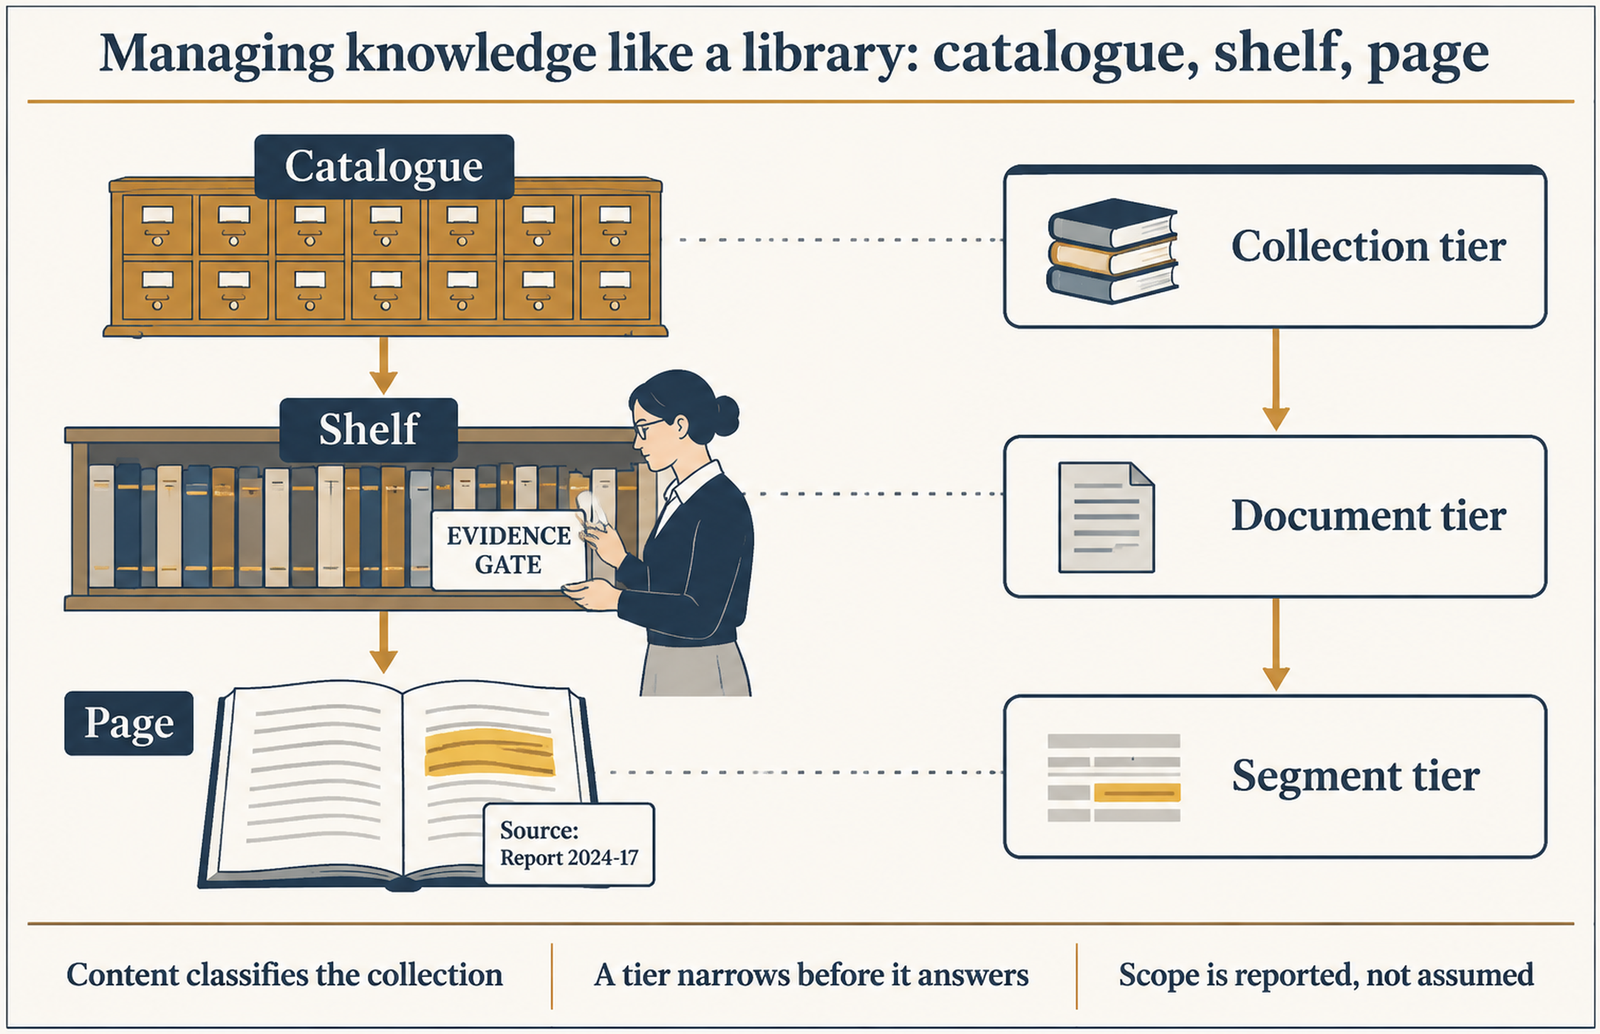
\includegraphics[width=\textwidth]{fig_analogy}
\caption{Design analogy: HMRS manages knowledge like a library. The catalogue, shelf and page stations correspond to the collection, document and segment tiers; the librarian's verification is the optional evidence gate. The three contracts (bottom) state what the management structure guarantees.}
\label{fig:levels}
\end{figure*}

\begin{figure*}[t]
\centering
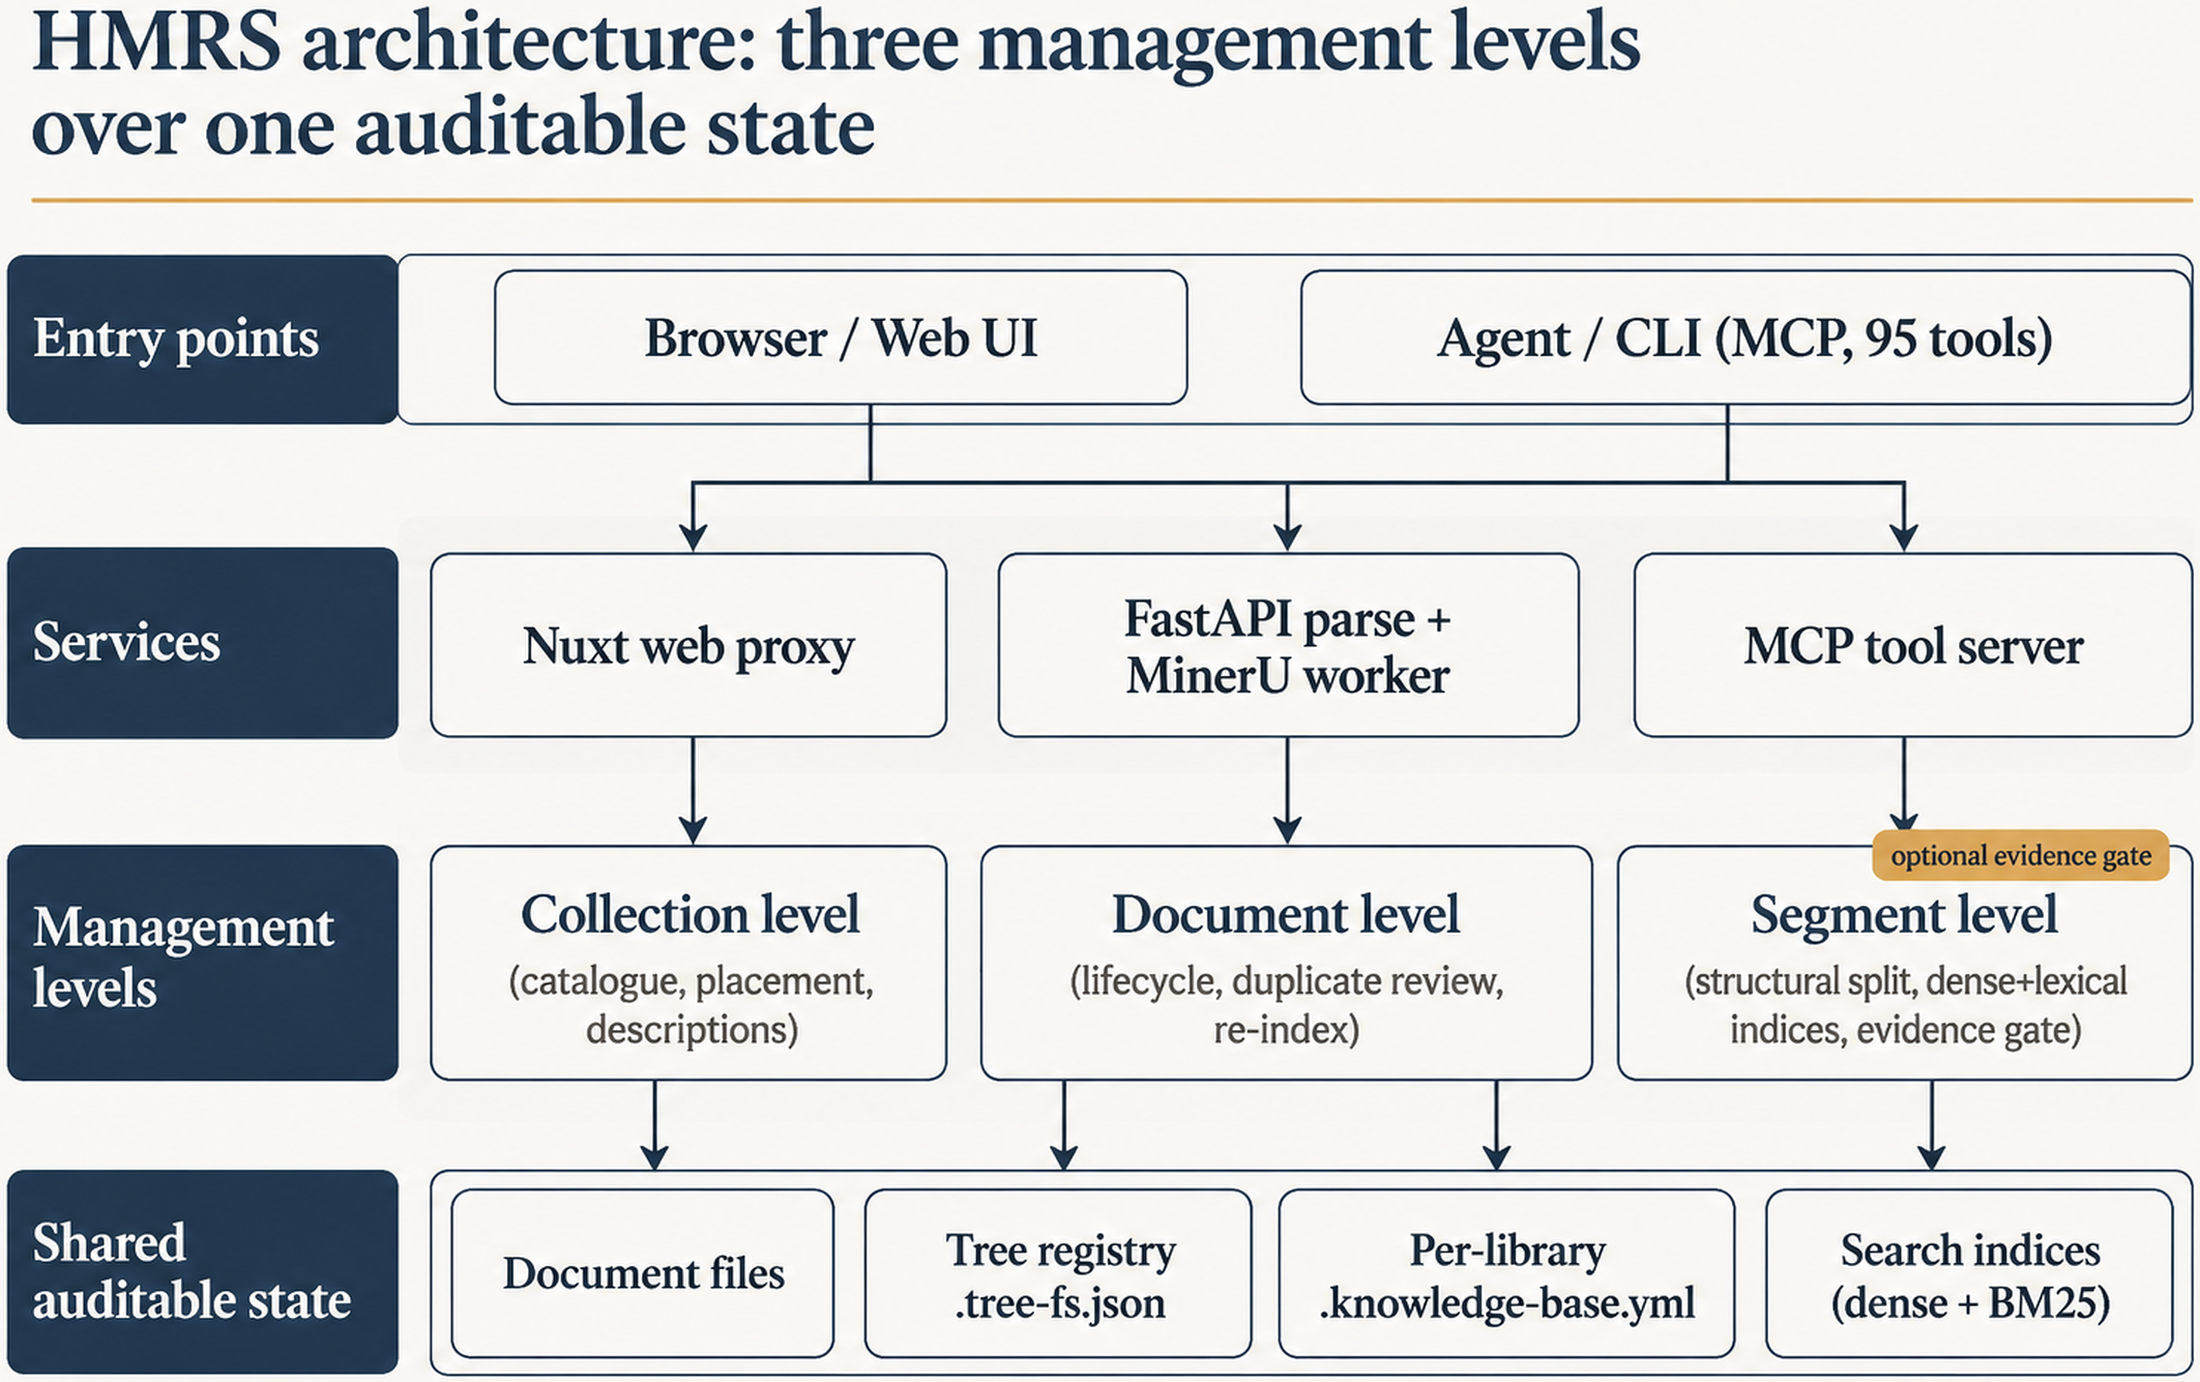
\includegraphics[width=\textwidth]{fig_architecture}
\caption{HMRS service architecture. Entry points (browser, agent/CLI) reach the Nuxt proxy, the FastAPI+MinerU parse service and the MCP tool server, which operate three management levels over one shared auditable state (document files, tree registry, per-library metadata, search indices). The evidence gate is an optional segment-level call.}
\label{fig:arch}
\end{figure*}

\begin{figure*}[t]
\centering
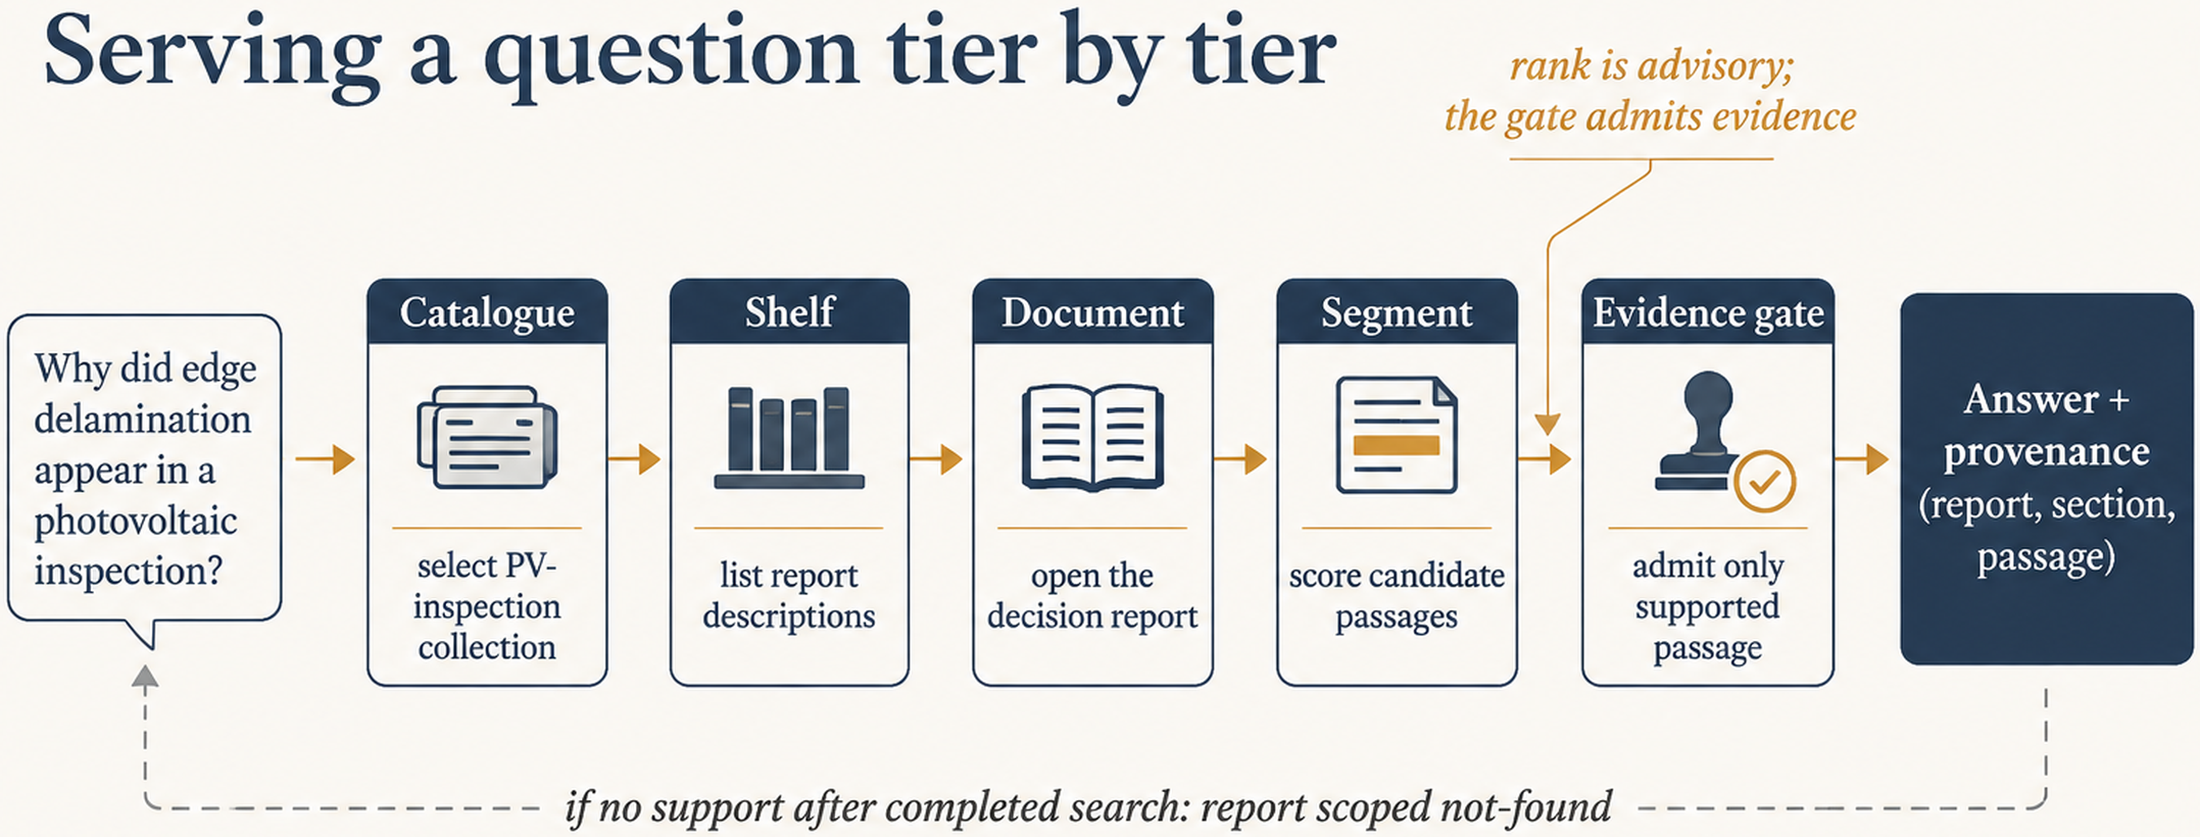
\includegraphics[width=\textwidth]{fig_workflow_demo}
\caption{Worked example of the tiered access path. A question narrows from catalogue to shelf to document to segment; the optional evidence gate admits only a supported passage and the answer carries provenance. A completed search without support yields a scoped not-found report.}
\label{fig:workflow}
\end{figure*}

Figure~\ref{fig:workflow} relates the acquisition and query workflows to
their shared state. The management path covers acquisition (Section~\ref{sec:acquisition}),
content-informed organisation and lifecycle checks
(Section~\ref{sec:organization}), and the tool and runtime layer
(Section~\ref{sec:implementation}). The chat endpoint defines pinned-search
and all-library librarian policies. Hybrid is a composed retrieval
configuration, not a third built-in server policy; it combines vector and
catalogue calls under an explicit directive. The document graph supports
navigation, not evidence. Experience retrieval and the persona-distillation workflows reuse
knowledge-base infrastructure but follow their own retrieval and filtering
paths; neither is described here as invoking Laya, and neither was evaluated
at scale.

The platform exposes five management domains: acquisition, organisation,
lifecycle, query and operational experience. Some controls are enforced by
API/MCP operations; semantic and quality checks are agent-workflow procedures,
and campaign audits test selected outcomes. Table~\ref{tab:functions}
distinguishes these layers and maps each domain to the evidence that exercises
it.

\begin{table*}[t]
\centering
\small
\setlength{\tabcolsep}{4pt}
\caption{Management functions, the enforcement or workflow check associated
with each, and the evaluation that exercises it. The table separates API/MCP
controls from agent procedures and campaign audits; semantic choices such as
which collection owns a document remain workflow decisions and are measured,
not enforced.}
\label{tab:functions}
\begin{tabular}{@{}>{\raggedright\arraybackslash}p{0.13\textwidth}>{\raggedright\arraybackslash}p{0.37\textwidth}>{\raggedright\arraybackslash}p{0.30\textwidth}>{\raggedright\arraybackslash}p{0.11\textwidth}@{}}
\toprule
Group & Operations & Platform or workflow check & Evidence\\
\midrule
Acquisition & submit, parse (MinerU), quality review, duplicate review, structural split, store, index & parse-task state; workflow quality checks; entry-point-specific deduplication and indexing; post-index probe & E1\\
Organisation & create library or sub-library, content-informed placement, descriptions and tags, duplicate review & API validates identifiers and required fields; workflow checks descriptions and tags; audit compares files, tree and library metadata & E1--E2\\
Lifecycle & move, rename, delete, force re-index, graph build & operation-specific API updates; reconciliation audit detects selected stale or inconsistent state & E2\\
Query & tier selection, vector, keyword, catalogue and two-stage search, gate invocation & endpoint enforces tool allow/deny lists, timeouts and turn limits; invoked gate returns survivor provenance & E4--E8\\
Experience & extract, approve, tier, search & experience tools apply their own retrieval, verification and credibility filters & E3\\
\bottomrule
\end{tabular}
\end{table*}

\subsection{Data model and object lifecycle}
\label{sec:datamodel}
\label{sec:lifecycle}

Documents are Markdown with extracted images. Library state is described by
the document files, the \texttt{.tree-fs.json} registry and each
\texttt{.knowledge-base.yml}. The ingest workflow tracks raw, parsed, stored
and indexed states and can mark completion after its configured retrieval
probe. Indexing is a separate transition: some save paths start vector/BM25
indexing asynchronously, while the web parsed-file save path does not.
Reconciliation detects selected stale-index conditions or disagreement among
the three sources; it is not a cross-store transaction. Because the three
sources are written by different management operations, the collection has no
single authoritative record of its own state, and the reconciliation audit
exists to make disagreement observable rather than to prevent it.

\section{Acquisition and automatic classification: from parsed document to
owned collection}
\label{sec:acquisition}

Acquisition determines what later retrieval can support, and it is where a
document is assigned to the collection that owns it. HMRS submits PDFs,
Office files and scans to MinerU through an asynchronous parsing service
\citep{mineru}; parse tasks return identifiers that callers poll to completion,
and OCR, layout and formula-extraction failures remain visible rather than
being stored as empty documents.

The intended ingest workflow follows observable stages: submit, parse,
agent-mediated quality review, duplicate decision, optional split, storage,
classification, indexing and a retrieval probe. Depending on the entry point,
artefacts may include a parse task identifier, a quality report, a content
fingerprint, a split manifest, a storage record, a placement decision and a
probe result. The workflow treats a content-derived retrieval probe as evidence
of retrievability; an HTTP success from a save call alone does not establish
that property. The platform accepts scanned pages, Office files and plain
text, but quality review, classification and completion checks are not all
enforced by the parse API.

\subsection{Quality gates and ingest lifecycle}

Duplicate handling has two paths rather than a universal admission gate. The
upload service rejects an exact same-parent duplicate by content hash, while
the separate near-duplicate tool reports similar candidates for review at a
configured threshold; it does not delete them automatically. In the ingest
workflow, an agent reviews parsed text for OCR noise, binary residue, bodyless
headings, whitespace collapse and language mismatch. Save and indexing behaviour
depends on the entry point: the web parsed-file save route stores content
without starting indexing, while the MCP parsed-document save operation can
start vector/BM25 indexing asynchronously. The ingestion agent classifies the document into a library whose scope matches
the parsed content's subject, not its filename, and the classification is
recorded so that the owning collection can be compared with the catalogue
afterwards.

When requested and above the configured context ceiling (30,000 characters in
the arXiv campaign; 60,000 in later configurations), documents are split at
recognised structural markers. The splitter targets 0.85 utilisation as a
soft target and detects units such as headings, Markdown tables, lists, block
quotes and fenced code. It does not guarantee preservation of equation
boundaries. Descriptions and tags are derived from the body and checked by the
ingest workflow; mismatches call for metadata correction, not document
rewriting.
Vector/BM25 indexing and graph construction are distinct operations.
Post-index verification checks selected properties such as a non-empty vector
collection and expected chunk identifiers; reconciliation can detect stale
index state, but is not a transaction across storage and index services.

\subsection{Acquisition evidence and accounting limits}

The 100-paper campaign produced 322 stored parts in five libraries, so the
collection level was populated across five distinct owning collections rather
than a single corpus.
Its reconciliation is incomplete: the state file records 91 submitted names;
at the 2026-10-13 evaluation snapshot 79 papers were retrievable and 21 were
not, and
the surviving artefacts do not enumerate attempts and failures per paper, so
the missing 21 cannot be attributed to parsing alone. Formula-dense scans and
a recovered batch-process crash were observed; neither establishes the cause
for every missing paper.

A separate cross-lingual test processed 400 Wikipedia pages per language:
ingestion success 1.0 in both rounds, and automatic membership accuracy 0.875
for English against 1.0 for Chinese and Japanese, which measures how often
content-based classification placed a document in the correct collection
independently of its filename, with the per-language storage and
self-retrieval results in Section~\ref{sec:e1}. These measurements
characterise ingestion, classification and storage, not answer quality.

\section{Collection and document management: organisation, classification and
lifecycle}
\label{sec:organization}

Organisation determines which collections exist, which tier can see a
document, and whether the stored state remains trustworthy. HMRS places
documents by content rather than filename; split parts inherit the source
assignment, and the catalogue exposes library and document descriptions
before full bodies are read. This section covers the collection and document
levels of Table~\ref{tab:levels}; the segment level is treated in
Section~\ref{sec:retrieval}.

\subsection{Classification, metadata, tags and duplicate review}
\label{sec:org-placement}
\label{sec:org-registries}
\label{sec:org-tags}
\label{sec:org-dedup}

Integrity checks compare the document files, the \texttt{.tree-fs.json} tree
and each library's \texttt{.knowledge-base.yml} for document existence, path
and index metadata. Tags derive from content and are checked against it.
Duplicate detection reports candidate pairs for review; deletion is not
automatic because adjacent parts may be similar while containing distinct
source sections.

The layer's operations are library and sub-library creation, classification,
description and tag edits, move, rename, delete, duplicate review and forced
re-index. Each operation updates the state relevant to it; for example, a move changes
the document path and registry entries, while re-indexing updates search
indices. The audit compares the files and registries where applicable. The catalogue lists libraries, their
descriptions, sub-library containers and document descriptions, which lets a
reader or an agent decide where to look before opening a body. Classification
is the one operation whose semantic choice is not mechanical: the ingest agent
selects the library from the parsed content, and the platform checks the
consequences rather than the choice. The same asymmetry holds at query time:
the tier that selects a collection is chosen by the workflow, whereas the
tiers that open, score and index a document are server operations.

Sub-libraries are tree nodes with their own descriptions and indices. Index writes resolve the document's owning library; searching a parent
library traverses its descendants' collections. This supports hierarchical
organisation without implying that child vectors are stored in the parent's
collection.

\subsection{Lifecycle operations, graph and operational knowledge}
\label{sec:org-lifecycle}
\label{sec:org-graph}
\label{sec:org-experience}

A historical rename trial left stale vector chunks until forced re-indexing.
The current rename path starts index synchronisation asynchronously, with
failures logged as non-fatal; checking the resulting index remains necessary
because successful metadata updates alone do not establish index consistency. The document graph supports navigation and candidate
expansion, not evidence. Operational lessons are stored as retrievable
documents with credibility tiers, but the available measurements are case
examples rather than a scale evaluation of distillation, approval or
credibility decay.

\subsection{Organisation contract}
\label{sec:org-integrity}
\label{sec:org-summary}

The evaluation checks three-source consistency, content-derived descriptions,
regression probes and lifecycle outcomes (Section~\ref{sec:e2}). The contract
makes stale or inconsistent state detectable; it does not prevent every
failure by construction. Merge and split remain outside the controlled test
scope, so performance claims must be read within the corpus sizes reported in
the Evaluation section.

\section{The tiered access path: from collection to admitted segment}
\label{sec:retrieval}
\label{sec:lanes}

The access path reads the collections, catalogue and indices maintained by
acquisition and organisation. It is the query-side counterpart of the
management levels: the catalogue tier chooses a collection, the shelf tier
chooses documents within it, the document tier opens a body, and the segment
tier scores its parts. Three access policies use different affordances of that
path, and a calling workflow may invoke the separate server-side Laya evidence
gate. The tool fetches referenced document text, segments it and applies a
local, query-conditioned verdict. Its model-card field (\texttt{noul}) is a
typed 0--1 score; this study reports no probability-calibration experiment and
does not interpret the score as a calibrated probability. Segments meeting the
configured threshold (0.5 by default) are returned as survivors with
provenance. A scored segment below the threshold is not admitted, while tool
or fetch failures are reported separately; a partially completed call may
still return successfully scored survivors. A scoped not-found report is
reserved for a completed search with no supporting evidence, not for an
execution failure.

An access workflow can combine the following operations. Their order and
inclusion depend on the entry point and the question; the list is not a
server-enforced sequence for every query.
\begin{enumerate}
\item \emph{Rewrite.} The agent forms retrieval queries from the question.
\item \emph{Gather.} A pinned search calls two-stage or vector search; a
catalogue-first search selects collections and document descriptions. A
composed workflow can combine candidates from more than one source.
\item \emph{Merge and cap.} Where multiple sources are combined, the workflow
can deduplicate and limit the candidate set. Specific limits are properties of
the evaluated configuration, not universal platform guarantees.
\item \emph{Judge.} When invoked, the gate fetches candidate documents, scores
segments and returns survivors with provenance; fetch and tool failures are
reported separately from low scores.
\item \emph{Read and answer.} The agent examines the evidence pack and may read
a surviving document to check a specific claim before synthesising an answer.
\end{enumerate}

\begin{algorithm}[t]
\caption{Tiered access with optional evidence gate}
\label{alg:tiered}
\begin{algorithmic}[1]
\Require question $q$; catalogue $\mathcal{C}$; threshold $\tau$; gate flag $g$
\State $D \gets \textsc{GatherCandidates}(q,\mathcal{C})$ \Comment{pinned or catalogue-first}
\If{$g$}
  \State $S \gets \textsc{LayaJudge}(D,q,\tau)$ \Comment{fetch, score and return survivors}
\Else
  \State $S \gets \textsc{ReadSelected}(D)$
\EndIf
\If{execution incomplete}
  \State \Return failure and searched scope
\ElsIf{completed review finds no support}
  \State \Return scoped not-found (searched scope, blind spots)
\Else
  \State \Return agent-synthesised answer with source references
\EndIf
\end{algorithmic}
\end{algorithm}
Exhausting a policy's call budget is intended to produce a scope and blind-spot
report. The endpoint enforces timeouts and turn limits; the per-policy budgets
are workflow instructions, not server quotas.

\subsection{Tier policies and the evidence gate}
\label{sec:trace}
\label{sec:gate}
\label{sec:gate-primitive}
\label{sec:twostage}

The current chat instructions provide two retrieval modes. In pinned mode,
the agent rewrites the question and calls the two-stage search (preferred) or
vector search within the selected collections; it can send candidate references
to Laya in sequential batches and optionally open a survivor for a specific
quote. In all-library mode, the instruction walks the catalogue and selected
shelves, selects document references from descriptions and sends these to Laya
before reading survivors. These are agent instructions, so actual tool use is
reported from traces rather than assumed from the instruction. Endpoint-level
timeouts and turn limits bound execution; retrieval sequences and batch sizes
are workflow instructions rather than separate server-enforced per-lane quotas.

The experiments also use fixed retrieval configurations. In particular, the
historical hybrid wrapper evaluated in Section~\ref{sec:e4} is no longer a
registered tool. Another controlled candidate-pool experiment uses per-library
vector top-30 at cosine threshold 0.35 together with catalogue candidates,
followed by fusion and a twelve-candidate cap. These values identify that
experiment, not the current chat default. A composed hybrid directive may call
vector and catalogue tools in an agent workflow. Table~\ref{tab:lanes}
summarises the current modes and the evaluated composition.

The gate is the local Laya evidence classifier \cite{laya}, exposed as
\path{kb_laya_judge}. In reference mode, the server fetches each document,
judges its segments and returns provenance with a bounded evidence pack. The
verdict controls admission, not truth; the verifier remains subject to
calibration and transport limitations.

\begin{table*}[t]
\centering
\small
\setlength{\tabcolsep}{5pt}
\caption{Access policies over the tiered path. Modes differ in how candidate collections and documents are selected.
The hybrid row describes an experimental composition.}
\label{tab:lanes}
\begin{tabular}{@{}>{\raggedright\arraybackslash}p{0.11\textwidth}>{\raggedright\arraybackslash}p{0.19\textwidth}>{\raggedright\arraybackslash}p{0.24\textwidth}>{\raggedright\arraybackslash}p{0.16\textwidth}>{\raggedright\arraybackslash}p{0.20\textwidth}@{}}
\toprule
Policy & Tiers traversed & Retrieval affordance & Budget type & Intended terminal report\\
\midrule
Search & pinned collections, segment & Two-stage or vector search & Endpoint turn limit & Answer or report not-found\\
Librarian & catalogue, shelf, document, segment & Catalogue navigation and optional judging & Workflow instructions & Scope and blind spots\\
Hybrid & catalogue and segment & Composed vector and catalogue calls & Configuration-specific candidate cap & Candidates or judged survivors\\
\bottomrule
\end{tabular}
\end{table*}

The two-stage tool builds a candidate pool with lexical search and optional
graph expansion, then applies dense ranking. It does not call the
evidence gate; a ranked chunk is not admissible evidence until verified, and a
similarity threshold is not an abstention mechanism. The 13 October catalogue
incident showed that oversized tool returns can conceal documents before
reasoning begins. The tested repair adds a server-side character budget,
grouped views and pagination; its behaviour is reported in the Evaluation
section.

\subsection{Honest abstention}
A candidate list may contain high-similarity but unsupported documents. The
answer workflow instructs the agent to report not-found when its completed
evidence review finds no support, including the searched scope and known blind
spots, rather than falling back to parametric knowledge. This behaviour was
observed in the reported trials; it is not a server-side semantic-classifier
guarantee. Timeouts, unavailable tools and incomplete searches are execution
failures, not evidence of semantic absence (Section~\ref{sec:eval}).

\section{Agent interface and implementation}
\label{sec:implementation}
\label{sec:impl}

\subsection{MCP tools and lane policy}
\label{sec:impl-tools}

The platform exposes MCP tools across management and retrieval categories. They
fall into the management groups of Table~\ref{tab:functions}: parsing and
quality review for admission, library and sub-library creation, placement,
description and tag editing for organisation, move, rename, delete and
forced re-index for lifecycle, catalogue, vector, keyword and two-stage
search for the access path, the Laya evidence gate for segment admission,
the document graph for navigation, and operational-experience tools, plus
persona-distillation workflows that are outside the scope of this evaluation
and use their own retrieval and synthesis path.
Access policies
receive read-oriented tool sets; administrative writes remain separate, and
long-running parse, re-index and graph operations return pollable task
identifiers. Fig.~S1 summarises the software design: a tool
layer over management services that share one auditable state, with the
evidence gate as an optional segment-level call.



The chat endpoint adapts multiple agent harnesses to the lane interface. The
server selects a harness and permission mode, enforces configured tool
allow/deny lists, applies endpoint timeouts and turn limits, and may register an
asynchronous task. Lane-specific retrieval sequences and call budgets are
workflow instructions; the endpoint does not enforce a separate per-lane call
quota.

\subsection{Runtime and deployment}
\label{sec:impl-runtime}

The backend uses Python 3.12 and FastAPI. ChromaDB stores cosine-space HNSW
collections with normalised BGE-M3 embeddings (1024 dimensions)
\cite{chroma,hnsw,bge-m3}; Neo4j stores the document graph \cite{neo4j};
BM25 supports lexical search \cite{bm25}; MinerU provides parsing and OCR
\cite{mineru}. The Laya verifier runs locally as a serialised worker.

The evaluation environment is one self-hosted Windows workstation with an
RTX 5060 (8 GB) used for embeddings and judging. Local execution reduces
external service dependencies but does not establish privacy, access-control or
multi-host deployment guarantees. The implementation and scripts are available
at \url{https://github.com/kingdol666/rag-knowledge}; experimental corpora
remain subject to their data-use constraints.

\section{Evaluation}
\label{sec:eval}
We evaluate the management lifecycle and retrieval on separate corpora. E1--E3
cover ingestion, organisation, scripted routing and experience; E4 and
Section~\ref{sec:ladder-opt} compare retrieval configurations; E5--E8 examine
answer behaviour, deployment, verification and operational boundaries. Results
are reported per corpus, without pooling. Table~S9 maps management functions
to tests; Table~\ref{tab:retrieval} and Table~\ref{tab:e5-answers} report
retrieval and answer checks.

\subsection{Experimental setup}
\label{sec:eval-setup}
\textbf{Corpora and questions.} The industrial demonstration corpus contains
42 documents in five libraries, including twenty near-duplicate telemetry
reports, and 16 developer-authored questions with gold document fragments; Q16
shares a token with its gold filename. The arXiv campaign submitted 100 papers
across about 25 domains, producing 322 stored parts in five libraries; 79 were
retrievable at the 2026-10-13 snapshot. Its ten gold questions are keyed by
arXiv identifiers. The cross-lingual ingestion corpus has 400 Wikipedia pages
per language (English, Chinese and Japanese) and 40 extractive queries per
language; its index self-check is not a task-level retrieval comparison. A
separate routing corpus has 138 documents in 879 parts across ten domains,
72 in-domain questions and four out-of-domain probes per arm; two
cross-placeholder probes are excluded. Questions and annotations are
researcher-authored, not sampled user queries.

\textbf{Measures and controls.} Document-level Hit@5, Recall@5 and MRR@5
measure the returned top five, with MRR zero if no gold is in that window
\cite{craswell-msmarco-2021}. Scripted route accuracy checks the gold-domain
label, whereas gold-string containment checks an exact substring in the
returned evidence; neither measures semantic answer correctness. The answer
grid measures gold-ID presence in answer or trace, lexical coverage of at
least $\lceil3n/5\rceil$ annotated terms, and citation-marker presence;
markers do not verify source resolution or entailment. Wilson intervals are
conditional on questions and a run; exact McNemar tests are exploratory and
unadjusted. Agent arms use one model and one run per condition; retries after
transport failures are not independent repeats. Two corpus-integrity defects
were repaired before measurement, so their natural failure rate is unknown.
Table~S10 summarises the experimental design and headline results.

\subsection{E1: Acquisition and parsing}
\label{sec:e1}
The 100-paper campaign recorded 322 parts. At the evaluation snapshot 91
paper names appeared in the ingest state and 79 papers were retrievable:
12 recorded and nine unrecorded papers were not retrievable. The records do
not establish individual parse status or the stage causing each failure. In
the cross-lingual benchmark ingestion succeeded in both rounds, and
membership against source-category labels was 0.875 for English and 1.0 for
Chinese and Japanese; the post-ingest Hit@1 is an index self-check, not a
retrieval benchmark. A separate 50-paper, 26-domain campaign parsed and
verified all papers, but 41 negative tag flags did not block ingestion.

\subsection{E2: Organisation, consistency, and management operations}
\label{sec:e2}
A disposable-library rename left stale chunks in the vector index: 18 instead
of nine, with duplicate results; forced re-index restored nine. The 322-part
campaign passed its content check on all parts and three-source checks on a
33-part sample. A disposable three-level fixture supported parent-to-child
moves, listing, reading and judging. Of 16 lifecycle scenarios, create, move,
delete and forced re-index passed, while task-status reporting and the update
check failed; merge and split were not controlled. Tag checking passed 165
parts, while orphan tags and one cross-library registry leak were observed.
The graph supplies navigation rather than evidentiary support.

\subsection{E2b: Paired route-card audit}
\label{sec:routing-audit}
A scripted route-card probe returned the labelled domain for 72/72 in-domain
questions in A0 and 37/72 in nominally name-only A3; 35 routes were correct
only in A0 (Figure~\ref{fig:routing}). This is not an independent LLM-agent
selection test. Although the A3 indexed cards excluded descriptions, an
unlogged fallback could read them; some questions share titles with route-card
descriptions. The difference therefore does not isolate the effect of
removing descriptions. Of the 72 questions, 52 were automatically expanded
and 47 came from three domains, limiting generality.

\begin{figure*}[t]
\centering
\includegraphics[width=\textwidth]{fig3_routing}
\caption{Paired scripted route audit (72 in-domain questions). (a) Gold-domain
choice: A0 72/72, A3 37/72 (Wilson 95\% intervals; McNemar
$p=5.82\times10^{-11}$). (b) Exact-string containment: A0/A3 Laya evidence
packs and A1 concatenated text from all 879 parts (37/72, 33/72, 72/72; Wilson
intervals; paired $p=0.4545$ for A0--A3 and $p=5.82\times10^{-11}$ for
A1--A0). (c) Trace-recorded text bytes on a symmetric-log axis linear through
1 KB, including 11 zero-byte A3 cases; (d) tool wall-clock on a log axis.
Boxes show IQR, whiskers 5th--95th percentiles, dots questions and diamonds
means. A0/A3 bytes sum candidate-snippet and evidence-pack text (possible
overlap); A1 sums document-read responses. Tool time excludes answer
generation. A1 is a script, not an answering agent; the A3 fallback is
unlogged. These are routing, substring and tool-cost diagnostics, not answer
quality or an isolated description effect.}
\label{fig:routing}
\end{figure*}


Evidence-pack containment was 37/72 for A0 and 33/72 for A3. A mechanical
read-all script found all 72 strings after reading 879 parts; it produced no
answers. It averaged 24.3 MB and 253.7 s across 897 calls per question, versus
31.4 KB and 16.3 s for A0. Recorded bytes may include overlapping text and are
neither network traffic nor measured model input; tool time excludes answer
generation. Read-all is a string-containment diagnostic, not a careful-reading
agent or answer-quality baseline. The follow-up content configurations are
reported in Section~\ref{sec:ladder-opt}.

%% n8b_eval.tex -- evaluation, middle part: E3 (operational knowledge and
%% automated distillation) and E4 (retrieval quality and the role of the
%% verdict). Compressed 2026-10-12. Labels owned here: sec:e3, sec:e4,
%% sec:eval-retrieval, tab:retrieval, tab:e4-modes, fig:retrieval,
%% fig:marginvariants.
\subsection{E3: Operational knowledge and automated distillation}
\label{sec:e3}

The experience store holds operational lessons as retrievable
documents---addressed, indexed and searched as an ordinary document, with a
credibility tier deciding whether it may be shown at all
(Section~\ref{sec:org-experience}). Three case measurements exist: an
extraction campaign over one small knowledge base produced thirteen
candidate drafts (archived \path{experience_smoke.json} in the 2026-10-13
batch tarball; \texttt{extract\_candidates}~13, \texttt{drafts\_created}~13);
one end-to-end scenario was sedimented into one experience
(\texttt{exp-d6f4d47ae3d6}) that a later global experience search returned
first, at local similarity 0.711 (archived scenario A6 of the 2026-10-12
full-test campaign); and the draft-approval path was never exercised, because
the draft pool was empty (\texttt{count}~0) and \path{experience_draft_read}
and \path{experience_draft_approve} could not run; the heuristic extraction
path had run only in dry-run mode, returning a dump the quality gate would
reject. One scenario and thirteen candidates cannot support an effectiveness
claim; scheduled distillation, review and approval at scale, application
feedback and credibility decay went unexercised. What they show is narrower:
an operational lesson can travel the document path with its tier attached.

\subsection{E4: Retrieval quality and the role of the verdict}
\label{sec:e4}
\label{sec:eval-retrieval}

Nine configurations, defined here so the table reads on its own. Five were
measured through their own tool-layer entry points: \emph{Dense} via
\texttt{kb\_search\_vector} with BGE-M3 \cite{bge-m3}; \emph{Graph} via
\texttt{kb\_graph\_search}, a keyword match over node names, paths and tags in
the document graph; \emph{Two-stage} via
\texttt{kb\_search\_two\_stage} (Section~\ref{sec:twostage}); and the hybrid
rows via \texttt{kb\_hybrid\_search}, an earlier server-side single-call
composition of the vector, catalogue and judging tools, with the gate off
(\emph{Fusion-only}) and on (\emph{HMRS-Hybrid}). \emph{BM25} runs in process
over the fetched full texts (jieba tokenizer, $k_1=1.5$, $b=0.75$), and
\emph{RRF} fuses that ranking with the dense one at $k=60$
\cite{rrf-cormack}; neither is the platform's keyword tool, so the millisecond
latencies are in-process measurements rather than a server round trip. The
evaluated hybrid wrapper is no longer registered in the current tool layer,
whose hybrid lane is the composed chat configuration of
Section~\ref{sec:twostage}, so the negative ordering result below is bounded
to that retired wrapper. Two further rows are derived offline by replaying the
judged hybrid run's logged twelve-candidate pools and verdict scores:
\emph{Judge-as-filter} keeps survivors in fusion order and \emph{RRF-fuse}
fuses the fusion ranking with the judge-score ranking at $k=60$. All three
see the same candidates and scores, so the comparison is an attribution,
not a benchmark. Because every logged candidate survived the configured 0.5
threshold, the filter replay is identical to fusion order by construction and
does not test filtering. Figure~\ref{fig:retrieval} renders the two corpora of
Table~\ref{tab:retrieval} so the quality and the cross-corpus pattern can be
read at a glance.

\begin{figure*}[t]
\centering
\includegraphics[width=\textwidth]{fig_retrieval_comparison}
\caption{Tool-layer retrieval quality on the two corpora of
Table~\ref{tab:retrieval}. (a)~The 42-document industrial demonstration corpus
over 16 gold-annotated questions: Hit@5, Recall@5 and MRR@5 for the seven
logged configurations. (b)~Hit@5 on the 79 retrievable arXiv papers over ten
questions. On the industrial corpus the evaluated, retired HMRS-Hybrid ordering is the
weakest configuration on all three metrics, while BM25 and RRF reach 1.00
Hit@5; on the arXiv corpus every configuration except Graph reaches 0.90.
The two derived replays (Judge-as-filter, RRF-fuse) are reported in
Table~\ref{tab:retrieval} and Fig.~S4 rather than
duplicated here. Values are read from the frozen result artefacts
(\protect\path{exp1\_summary.json}, \protect\path{exp10\_papers\_toollayer.json}).}
\label{fig:retrieval}
\end{figure*}

\begin{table*}[t]
\centering
\small
\setlength{\tabcolsep}{3pt}
\caption{Tool-layer retrieval on the 42-document industrial demonstration corpus
(mean over 16 gold-annotated questions; top-5 document lists; latency per
call, warmed). The paraphrase column re-asks those sixteen questions in
different words (\protect\path{paper-kbs/experiments/results/exp6_paraphrase.json});
block~(b) repeats the Hit@5 measurement on a second corpus, the 79 retrievable
papers of the 100-paper arXiv ingestion, over ten questions.}
\label{tab:retrieval}
\resizebox{\textwidth}{!}{%
\footnotesize
\begin{tabular}{lcccccc}
\toprule
Method & Hit@5 & Recall@5 & MRR@5 & Paraphrase Hit@5 & Latency (mean) & Latency (median) \\
\midrule
BM25                  & 1.00 & 1.00 & 0.958 & 0.88 & 0.9\,ms    & 1\,ms \\
Dense (BGE-M3)        & 0.94 & 0.94 & 0.856 & 0.94 & 18\,ms     & 17\,ms \\
RRF (BM25$\|$Dense)   & 1.00 & 1.00 & 0.927 & 0.88 & 11\,ms     & 9\,ms \\
Graph (Neo4j)         & 0.56 & 0.53 & 0.562 & 0.56 & 68\,ms     & 68\,ms \\
Two-stage             & 1.00 & 0.97 & 0.927 & 0.94 & 77\,ms     & 40\,ms \\
Fusion-only           & 0.94 & 0.94 & 0.856 & 0.94 & 62\,ms     & 66\,ms \\
HMRS-Hybrid          & 0.44 & 0.41 & 0.226 & 0.50 & 542\,ms    & 582\,ms \\
\midrule
\multicolumn{7}{l}{\emph{Derived (offline, same logged hybrid pools):}}\\
\quad Judge-as-filter$^{\dagger}$ & 0.94 & 0.94 & 0.856 & 0.94 & \multicolumn{2}{l}{$^{\dagger}$542\,ms / 582\,ms} \\
\quad RRF-fuse & 0.88 & 0.88 & 0.606 & 0.88 & \multicolumn{2}{l}{(same single call)} \\
\bottomrule
\end{tabular}}
\par\smallskip
\raggedright\small
$^{\dagger}$\,Derived rows replay the HMRS-Hybrid run's own logged
12-candidate pools and judge scores, so they reuse that call's latency; the
judge executes once either way.

\par\smallskip
\resizebox{\textwidth}{!}{%
\begin{tabular}{@{}lcccccccc@{}}
\toprule
\multicolumn{9}{@{}l}{\textbf{(b)} Second corpus: 79 retrievable arXiv papers of the 100 submitted, ten questions}\\
\midrule
Configuration & BM25 & Dense & RRF & Graph & Two-stage & Fusion-only & HMRS-Hybrid & Judge-as-filter \\
Hit@5 & 0.90 & 0.90 & 0.90 & 0.20 & 0.90 & 0.90 & 0.90 & 0.90 \\
\bottomrule
\end{tabular}}
\end{table*}

The 42-document results show strong lexical retrieval: BM25 and RRF each
reached Hit@5 1.00, while the retired HMRS-Hybrid wrapper reached 0.44.
Excluding Q16, whose filename shares a question token, leaves BM25 at 1.00
on 15 questions. Baseline latencies are in-process and not comparable to a
server round trip. The 79-paper evaluation gives Hit@5 0.90 for seven of
eight configurations and 0.20 for Graph; its corpus and questions differ.

On identical logged candidate pools, the judge-score ordering yields Hit@5
0.44; keeping the original fusion order among recorded survivors yields 0.94.
All 191 recorded scores exceeded the 0.5 threshold, and one additional
candidate had no recorded score. Thus the observed loss concerns ordering;
the configured filter did not reject a scored candidate and its efficacy is
not established. The same-pool replay is a diagnostic of this retired wrapper,
not a benchmark of the current composed hybrid lane. Under paraphrase, the
judged configuration reached Hit@5 0.50 versus 0.94 with fusion order.
On the second corpus, Hit@5 did not fall but MRR fell from 0.90 to 0.70;
different corpus characteristics prevent causal attribution. See
Section~\ref{sec:e6} for the score distribution and Fig.~S4 for additional
replays.

\subsection{E4b: Content-layer configuration comparison}
\label{sec:ladder-opt}
The routing corpus was also used to compare eight evidence configurations.
A0 is the tiered baseline; A0f uses expanded document windows, A0h additionally
unions vector chunk windows, PD uses a navigation-free precise per-document
search, A1b a scoped flat union and reference-mode judge, A2 skips that judge,
A3 uses nominally name-only cards, and read-all scans every stored part.
A0h, PD and A1b differ in multiple components, so their differences cannot be
assigned to navigation alone. A3 may retrieve outside the evaluation scope.

In the 11 November aggregate, gold strings were contained for A0/A0f/A0h/PD/
A1b/A2/A3/read-all in 37/45/52/46/39/25/33/72 of 72 questions, respectively
(Figure~\ref{fig:ladder}); these are evidence-string proxies, not answer
correctness. Supplementary Tables S12--S13 give the per-arm intervals and
paired records. The A0h Wilson 95\% interval is [0.610, 0.812]. In exploratory,
unadjusted paired records, A0h contained the string while A1b did not on 13
questions and the reverse occurred on none (two-sided exact McNemar
$p=0.00024$). A0h led PD on seven questions while PD led on one
($p=0.0703$). These records do not show a statistically resolved advantage
over PD and are not unbiased deployment estimates: A0, A1b and A3 can use
the gold domain to resolve judge references, with unknown frequency and impact.

A later same-question record yields 39/44/51/45/39/25 for the first six arms,
respectively. Per-question agreement with the frozen record is 94.4\% for A0,
98.6\% for A0f, A0h and PD, and 100\% for A1b and A2; the same question set
is reused and complete execution provenance is unavailable. In a separately
added later A3 record, containment is 25/72, with 13 missing top candidates
and 23 empty packs; their causes are not established. Later read-all is
incomplete. The frozen read-all is a mechanical substring scan, not an agent
that reads and answers. A0h recorded 309 KB and 13.8 s per question versus
24.3 MB and 253.7 s for that scan; the recorded-byte definitions differ and
may include overlap.

Among A0's 35 misses, A0f, A0h and PD contain the string in 8, 15 and 9 cases,
respectively. These sets overlap and are not additive. A post-hoc search
classified five first matching string locations outside a nominal window and
30 inside; the chosen matching file need not be the gold document or a
candidate actually read, so these categories do not identify the causes of
misses (Figure~\ref{fig:miss-overlap}).

\begin{figure*}[t]
\centering
\includegraphics[width=\textwidth]{fig_ladder_optimization}
\caption{Content-layer optimisation arms on the 72 in-domain questions of the
ten-domain corpus. (a)~Blue circles and Wilson 95\% intervals show the
11 November frozen aggregate of gold-string containment; orange triangles
show later records on the same questions. The frozen aggregate combines runs
on different dates; A3 was added separately to the later record. Read-all is
incomplete in the later record. The dashed line is the frozen tiered baseline A0. A0f
(expanded-window judge) and A0h (plus a chunk-window union) have higher containment than A0; PD
(precise per-document, no navigation) is the ladder-versus-precise contrast
(A0h vs PD: 7--1 discordant, McNemar $p=0.0703$); A0h vs the scoped flat union
A1b is 13--0 ($p=0.00024$). A1b, A2 (no gate) and A3 (name-only cards) are the
flat and ablated controls; read-all is a mechanical upper bound, not an agent
baseline. A1b uses a reference-mode judge and can use the gold domain in
reference resolution; A0h and PD differ in both routing and chunk union.
(b)~Frozen-aggregate mean total tool calls and trace-recorded kilobytes per
question; bytes can include overlapping text.}
\label{fig:ladder}
\end{figure*}

\begin{figure}[t]
\centering
\includegraphics[width=\columnwidth]{fig_miss_overlap}
\caption{Overlap among configurations for the 35 questions where frozen A0
lacked the gold string. Each bar is a mutually exclusive outcome across A0f,
A0h and PD; the counts are not additive configuration gains. These are
substring results, not identified causes of failure.}
\label{fig:miss-overlap}
\end{figure}

\subsection{E5: Answer quality, abstention and cost}
\label{sec:e5}
\label{sec:agentic}\label{sec:abstention}\label{sec:composition}\label{sec:eval-agent}
Two ten-question grids compare a platform agent (P), direct file tools (F)
and a dense-search arm (D). The original grid uses different substrates; the
later grid pins the same five libraries. Gold-ID presence, strict and
alias-aware keyword coverage, and citation markers are deterministic checks,
not assessments of semantic support. A marker does not establish that a cited
passage exists or entails the answer.

\begin{table*}[t]
\centering
\footnotesize
\setlength{\tabcolsep}{3pt}
\caption{Answer quality per question and per interface in the original grid
(30 answer cells from \protect\path{run-20261013T094350Z-5f9faac}); the
controlled replication on a common substrate is reported in the text and adds
no column. The gold-ID check searches the answer or recorded trace and passes
10/10 cells in each arm; the column is not repeated. Each
arm column gives strict keyword coverage (\yes\ or $\times$), alias-aware coverage,
and the number of recognised citation markers (m). Strict coverage is a
majority rule on the annotated terms, not an all-terms rule. The column m counts
markers; the prose's 9/10, 7/10 and 2/10 count answers with at least one.
Markers do not establish that a cited section exists or supports the sentence
citing it.}
\label{tab:e5-answers}
\begin{tabular}{@{}l>{\raggedright\arraybackslash}p{0.335\textwidth}l*{9}{c}@{}}
\toprule
 & & & \multicolumn{3}{c}{Platform (P)} & \multicolumn{3}{c}{File tools (F)} & \multicolumn{3}{c}{Dense (D)}\\
\cmidrule(lr){4-6}\cmidrule(lr){7-9}\cmidrule(lr){10-12}
Q & Question (abridged) & Gold & s & a & m & s & a & m & s & a & m\\
\midrule
BQ01 & Transformer attention; why recurrence is replaced & 1706.03762 & \yes & \yes & 6 & \yes & \yes & 0 & \yes & \yes & 5\\
BQ02 & NISQ definition and its central limitation & 1801.00862 & \yes & \yes & 4 & \yes & \yes & 3 & \yes & \yes & 0\\
BQ03 & MultiMedQA and Flan-PaLM on MedQA & 2212.13138 & \yes & \yes & 4 & \yes & \yes & 1 & \yes & \yes & 1\\
BQ04 & Three ontologies subdividing the Gene Ontology & 1602.01876 & \yes & \yes & 1 & \yes & \yes & 1 & \yes & \yes & 0\\
BQ05 & European growth versus Unified Growth Theory & 1512.08067 & \yes & \yes & 0 & \yes & \yes & 0 & \yes & \yes & 0\\
BQ06 & Contributions governing precipitation extremes & 1503.07557 & $\times$ & \yes & 6 & \yes & \yes & 4 & \yes & \yes & 0\\
BQ07 & MameLoshnLM and its parameter scale & 2608.05850 & \yes & \yes & 1 & \yes & \yes & 2 & \yes & \yes & 0\\
BQ08 & Oxygen redox and cathode capacity & 2408.09942 & \yes & \yes & 2 & \yes & \yes & 0 & \yes & \yes & 0\\
BQ09 & Visual SLAM in dynamic scenes (MLP-SLAM) & 2410.10669 & \yes & \yes & 2 & $\times$ & \yes & 6 & \yes & \yes & 0\\
BQ10 & Tumour control under immune evasion & 2604.01385 & \yes & \yes & 3 & \yes & \yes & 6 & $\times$ & \yes & 0\\
\midrule
 & \emph{All ten questions} & & 9 & 10 & 29 & 9 & 10 & 23 & 9 & 10 & 6\\
\bottomrule
\end{tabular}
\end{table*}


In each arm the answer or recorded trace contained a gold identifier in all
ten cells in both grids. In the
original grid strict keyword coverage was 9/10 for each arm, alias-aware
coverage 10/10, and marker-bearing answers 9/10, 7/10 and 2/10 for P, F and
D (Table~\ref{tab:e5-answers}). Under the common substrate these marker
counts were 9/10 for each arm; strict coverage was 7/10, 7/10 and 8/10,
respectively. The substrate difference prevents attributing the marker gap to
an interface alone. Original-grid mean time and cost were 52.6 s and $\$0.711$
for P, 22.2 s and $\$0.487$ for F, and 24.5 s and $\$0.527$ for D; these are
single-run observations. The detailed source-presence audit appears in
Tables~S7--S8 and is not an entailment test.

\textbf{Answer-level case study.} A separate recorded demonstration parsed and
ingested a DeepSeek-R1 paper, then used two agent harnesses on the same four
questions. The case compendium reports eight responses checked against the
source on answer content, document provenance, quoted material and fabricated
facts; all eight passed that case review. This is a small, non-blinded case
study, not an independent benchmark of semantic answer accuracy (Table S14). On the
question asking for electricity cost, both responses said that the paper did
not provide an electricity figure and distinguished the reported $\$294$K
GPU-rental-based training-cost estimate. This is an observed refusal to infer
the requested absent value, not a general abstention guarantee. Three other
out-of-corpus probes over the industrial corpus also returned explicit
not-found reports; the retrieval threshold retained candidates in related
absent probes (Fig.~S3).

\subsection{E5b: Deployment-layer system arms through the public API}
\label{sec:sysarms}
Three questions crossed pinned, unpinned and pinned hybrid-directed API arms.
The pinned arms returned the two in-corpus gold identifiers, and all three
reported not-found for the out-of-corpus probe. In one unpinned setting, a
131-document, 74.9 KB catalogue exceeded the tool-output budget; a truncated
preview led to false refusal or a hang. After pagination and grouped views were
added, selected reruns completed, including the formerly failing query. These
observations do not establish general transport reliability. An eighteen-arm
honesty battery observed no fabricated citations in its final responses;
interrupted arms were rerun and each arm has one final observation.

\subsection{E6: When the verifier fails}
\label{sec:e6}
\label{sec:inflation}\label{sec:eval-verify}
The 191 recorded candidate scores from 16 hybrid runs include 17 in-pool
golds and 174 non-golds. All exceed the 0.5 threshold; an additional Q14
candidate has no recorded score. Gold and non-gold medians were 0.88 and
0.86 (Figure~\ref{fig:inflation}). The candidate-level Mann--Whitney test
ignores clustering by query, so its $p$ value is exploratory. Re-ranking on
these scores reduced Hit@5 to 7/16 versus 15/16 when recorded survivors
retained fusion order; a Q2 example appears in Fig.~S5.

\begin{figure}[!t]
\centering
\includegraphics[width=\columnwidth]{fig4_inflation}
\caption{Recorded Laya scores for 191 candidates from sixteen hybrid runs:
17 in-pool golds and 174 non-golds. All recorded values exceed the dashed
0.5 threshold; one additional Q14 fusion candidate has no recorded score and
its status is unknown. Group medians (0.88 gold, 0.86 non-gold) are not
distinguishable by a two-sided Mann--Whitney test ($p=0.26$). Horizontal
jitter is for legibility.}
\label{fig:inflation}
\end{figure}


A replay of the same pairs with an NLI checkpoint produced Hit@5 0.3125; a
span-level replay produced 0.1875. These results neither isolate truncation
nor prove the cause of verifier failure. The arXiv corpus did not show the
same top-five collapse; domain, language and corpus size changed together.
No answer-level test validates a higher filtering threshold.

\subsection{E7: Non-functional behaviour}
\label{sec:e7}
A 27-cell stability campaign completed without recorded answer errors across
three tasks, three lanes and three rounds. On one instance, a concurrency
sweep of 90/180/270 requests at 5/15/30 clients raised median latency from
5.2 to 1577 ms; 111 of 270 requests timed out at 30 clients. A later cache
repair lowered selected 30-client read-ladder median latency to 65.8 ms, but
the full sweep was not repeated. These are single-instance measurements;
raw concurrent-write counts and crash-recovery evidence were unavailable.

\subsection{E8: Ablations of the verification gate and the search scope}
\label{sec:e8}
A reconstructed fixed-candidate gate comparison used ten questions, a
12-candidate cap and a 4,000-character pack. All three arms packed the gold
first for eight gold-answerable questions; for nine of ten questions the
filtered and unfiltered document sets matched. LLM grades still varied under
identical packs (including $0\to5$ and $3\to0$); these observations do not
establish an answer-quality benefit from gating. The two non-gold questions
were abstained on in every arm. In the separate four out-of-domain routing
probes, the judge-survivor lists were empty in 2/4 A0 and 0/4 A0h cases.
Both A0 empty cases lacked a top candidate; these are neither verified gate
rejections nor answer-level refusal rates.

The scope diagnostic on the arXiv question set supplied the gold library to a
pinned condition, yielding Hit@5 1.0; a deliberately wrong library yielded
0.0. The unscoped search covered 20 live libraries, including 15 outside the
five-library evaluation corpus, and is not a matched-scope comparison. The
catalogue route selected the correct library first for six of eight
answerable questions; file names carried domain prefixes. These small,
single-engine experiments do not establish an independent effect of content
placement or an overall system advantage.

\section{Discussion and lessons learned}
\label{sec:discussion}

The management evaluation exposes both useful checks and their limits. In the
100-paper campaign, 79 submissions were retrievable and 21 were not; the
surviving records do not locate each failure. Automatic collection membership
was 0.875 for English and 1.0 for Chinese and Japanese. Of 16 lifecycle
scenarios, create, move, delete and forced re-index passed, whereas task-status
reporting and update checks failed. A historical rename test exposed a stale
index; current rename attempts asynchronous index synchronisation, whose
success still needs checking. These results motivate reconciliation without
establishing its completeness.

The scripted route audit hit the gold collection in 72/72 cases for A0 and
37/72 for nominally name-only A3. An unlogged fallback may use descriptions,
so this does not isolate their effect or measure independent agent routing.
The 72-question content-layer contrasts also change multiple components, and a
candidate-reference lookup in A0, A1b and A3 may depend on the gold domain.
They describe these records rather than a causal navigation benefit. The
mechanical full-read script located all strings in 879 parts but generated no
answers. Gold-string containment and the saturated gold-ID answer grids do not
establish semantic correctness or claim support.

Retrieval results do not establish consistent hybrid superiority. On the
42-document corpus, BM25 Hit@5 was 1.00 and the tested historical hybrid
wrapper achieved 0.44; on the 79-paper corpus the non-graph configurations
were at 0.90. On identical logged pools, verifier-score ordering reduced Hit@5
from 0.94 to 0.44, whereas fusion order restored 0.94. All 191 recorded scores
exceeded the configured threshold, so filtering did not activate and its
benefit was not measured. This is a bounded warning about a particular
ordering, not a finding about every verifier or current retrieval lane.

The reported answer and refusal cases show selected workflow behaviour, not a
reliable abstention rate. Pagination repaired selected oversized catalogue
paths, but incomplete searches and tool failures remain distinct from a
completed search without support. Stronger claims need independent questions,
controlled single-factor comparisons, repeated runs, semantic support review,
and tests of operations and recovery beyond the present local setting.

\section{Threats to validity}
\label{sec:threats}

\noindent\textbf{Data and scope.} The corpora and questions are small and
bounded; questions and gold annotations were developer-authored. The
72-question route set includes 52 automatically expanded questions, and 47
questions come from three English domains. Four out-of-domain probes cannot
estimate abstention rates. The storage reconciliation checks 33 of 322 parts.
Different retrieval arms and baselines use different scopes or substrates;
the historical hybrid wrapper, not the current composed hybrid lane, was
tested. Broader generalisation requires independent questions, larger corpora
and matched lexical and hybrid baselines.

\noindent\textbf{Measurement and comparisons.} Gold-string containment is a
substring proxy, not semantic answer correctness. Gold-ID, lexical and citation
marker checks likewise do not establish claim-to-source support. Two answer
grids used ten questions, one model and one run per arm; one replication held
libraries fixed, while substrates differed in the original grid. The scripted
full-read baseline searches strings and generates no answer. A0h, A1b and PD
change multiple components, and A0, A1b and A3 may use the gold domain to
resolve candidate references. Historical traces do not quantify this fallback.
A3 can also admit candidates outside the evaluated libraries and its
name-only routing may fall back to descriptions. Thus these arms cannot isolate
navigation or establish deployed performance. The later run repeats the same
questions and is not an independent test set; code hashes and judge inputs are
not fully preserved for each historical record.

\noindent\textbf{Statistical and operational validity.} Paired tests are
exploratory and not pre-registered; Wilson intervals condition on the sampled
questions and do not capture run-to-run variance. Candidate- and span-level
tests treat observations within queries as independent and may be
anti-conservative. Some reference-mode score and candidate inputs were not
retained. The manual refusal battery has one final observation per arm, and
experience approval was not exercised. The 16 lifecycle assertions, selected
pagination checks and one-workstation concurrency measurements do not establish
multi-host reliability, adversarial security, human adoption or crash recovery.
Future work should instrument the reference lookup, remove gold-dependent
fallback, conduct matched single-factor ablations and a genuine agent full-read
baseline, and pre-specify repeated comparisons and multiplicity control.

\section{Conclusion}
\label{sec:conclusion}

HMRS manages documents at three levels and answers questions along a path that
mirrors them. At the collection level, documents are parsed, classified into
the library whose scope matches their body, and catalogued with derived
descriptions and tags; at the document level, the collection is kept
consistent through move, rename, delete and forced re-index, with three
independent sources available for reconciliation; at the segment level, the
passages that may support a claim are scored and admitted with provenance.
Retrieval algorithms appear only at the lower two tiers, and the tier that
decides which collection is consulted is a management decision rather than a
ranking result.

The campaigns confirm selected paths of that structure and also expose its
limits. Ingestion and classification produced 322 stored parts across five
libraries, but 21 of 100 submissions were not retrievable and the surviving
records cannot attribute the failure to a stage. A separate 33-part storage
sample passed, while an independent disposable-library test exposed a
stale-index rename defect corrected by forced re-indexing. In 16 lifecycle
scenarios, create, move, delete and forced re-index passed, whereas task-status
reporting and the update check failed. The route-card audit found
collection-selection correctness of 72/72 and 37/72, but an unlogged fallback
rules out a causal interpretation. Evidence-pack string containment was
37/72 versus 33/72 ($p=0.4545$). A mechanical full-read script found all 72
strings after reading 879 parts, but generated no answers. The answer grids had
gold identifiers in the answer or recorded trace for all 60 cells, but lexical and citation markers do not
establish semantic support. On identical pools, verifier re-ranking reduced
Hit@5 from 0.94 to 0.44; fusion order restored 0.94, and the configured
threshold rejected none of 191 scores. On the same 72-question corpus, the
tiered path with a chunk-window evidence union contained the gold string in
52/72, above a scoped flat union with a potentially gold-dependent reference
lookup (39/72; 13--0, unadjusted $p=0.00024$) and above a precise arm without navigation (46/72;
$p=0.0703$).

These results document an auditable management structure, bounded per-tier
measurements and a deployment warning against verifier-as-ranker. The
content-layer comparisons change multiple components, and the flat arm uses a
potentially gold-label-dependent lookup; they do not isolate a hierarchy effect. They
do not establish system-level superiority, general retrieval effectiveness,
semantic answer quality or reliability. Broader evaluation needs independently
authored questions, repeated agent trials with run-to-run variance estimates,
claim-level support review, larger and repeated versions of the
ladder-versus-flat-and-precise contrast with multiplicity control, and
crash-recovery tests. Within these bounds, HMRS shows that treating the
collection as a managed, auditable object is a viable, inspectable basis for
evidence-traced retrieval.

%% n_back.tex — back matter, included by main_20p.tex after n11_conclusion.tex
%% and before the bibliography. This file is the single source of truth for
%% every declaration; n11_conclusion.tex carries the Conclusion and nothing else.
%%
%% The declarations follow the Conclusion. Keep the generative-AI statement
%% immediately before the references, pending a final check of the current KBS
%% Guide for Authors.
%%
%% AUTHOR ACTION: replace the CRediT names, confirm the funding wording, and
%% adjust or remove the acknowledgements.

\section*{CRediT authorship contribution statement}
\textbf{Author 1:} Conceptualisation, Methodology, Software, Investigation,
Data curation, Writing -- original draft. \textbf{Author 2:} Validation,
Writing -- review \& editing, Supervision. %% AUTHOR ACTION: adjust.

\section*{Declaration of competing interest}
The authors declare that they have no known competing financial interests
or personal relationships that could have appeared to influence the work
reported in this paper.

\section*{Funding}
This research did not receive any specific grant from funding agencies in
the public, commercial, or not-for-profit sectors. %% AUTHOR ACTION

\section*{Ethics statement}
This article does not report studies involving human participants, human
data, or animals.

\section*{Data availability}
Source code and benchmark scripts are available at
\url{https://github.com/kingdol666/rag-knowledge}. The repository indexes the
artefact inventory; hashes for the corrected and pre-correction annotations
and grader are recorded in
\path{paper-kbs/tex/journal_20p/revision-20261112.sha256}.
The supplement contains campaign inventories, per-question summaries and
lifecycle and ablation tables. November 2026 route traces are not public;
the authors retain them for requests subject to source-document restrictions.
The 42-document industrial corpus is a non-customer demonstration instance,
not deposited publicly. The verifier comparison is reproducible from the
released scores, golds and grader; an end-to-end rerun needs a substitute
corpus, with a recipe and synthetic sample in
\path{paper-kbs/notes/industrial-corpus-substitute-recipe-2026-10-16.md}.
% Author action: decide whether de-identified route traces can be deposited
% before submission. Kept as a source comment so no note is typeset in the article.

\section*{Acknowledgments}
The authors thank the maintainers of the open-source components the platform
builds on. %% AUTHOR ACTION: adjust or remove.

%% AUTHOR ACTION: confirm all service names and versions before submission.
\section*{Declaration of generative AI and AI-assisted technologies in the manuscript preparation process}
The authors used Anthropic Claude Code and ZCode, OpenAI Codex, and an AI image
generation tool for experiment execution, tabulation, language editing and initial figure
design. Figure concepts were reconstructed as editable vector diagrams. The
authors reviewed the final text and figures and take responsibility for them;
all reported experimental numbers come from logged runs on the authors'
machine.


{\fontsize{8pt}{9.5pt}\selectfont
%% References follow elsarticle-num at 8 pt finished type (raised from 7.2 pt
%% after review); page budget is managed by content, not by sub-baseline type.
\setlength{\bibsep}{0.3pt plus 0.1ex}
\setlength{\baselineskip}{8.6pt}
\urlstyle{same}
\bibliographystyle{elsarticle-num}
\bibliography{refs,refs_new_verified}
}

\end{document}
